\documentclass[a4paper]{article}
\usepackage[utf8]{inputenc}
\usepackage{fancyhdr}
\usepackage{geometry}
\usepackage{listings}
\usepackage{graphicx}
\usepackage{algorithmic}
\usepackage{float}
\usepackage{hyperref}

\lstset{
    language=Python,
    breaklines=true,
    numbers=left,
    frame=lines
}

\pagestyle{fancyplain}


\title{User Manual}
\author{Harry Milne}
\date{March 2014}

\lhead{Harry Milne}
\chead{Candidate Number: 2677}
\rhead{Centre Number: 22169}

\rfoot{\thepage}
\cfoot{}

\begin{document}
\maketitle
\tableofcontents
\newpage

\section{Introduction}

    The intended audience of this system is a normal household, in this case it is Paul Milne's household. Paul himself is very experienced
    in computing, however the rest of the household have an average IT knowledge.

    The purpose of the system is to provide an easy method to interface with the alarms; to turn them on and off. 

\section{Installation}
    \subsection{Prerequisites}

        \subsubsection{Hardware}

            \begin{itemize}
                \item Computer network within intended house
                \item Computer with camera attached for client
            \end{itemize}

        \subsubsection{Software}
            \begin{itemize}
                \item Python 2.7
                \item Qt UI Library
                \item SimpleCV
            \end{itemize}

    \subsection{System Installation}
        If you do not already have the files they are available for download at: \url{https://github.com/harrymilne/face_recognition_a2}.
        This repository has two root folders, `code' and `docs', Python files for the running of the client and server are under code.
        Once you are in the code directory this then has 3 folders, `client', `db\_browser' and `server', the `server' and `db\_browser'
        folders need to be on the same computer, whereas the client needs to be placed on a computer with access to a network capable of
        connecting to the computer which has the `server' and `db\_browser' folders on. 

    \subsubsection{Client}
        The client software must be installed anywhere you want end-users to be able to control the system, the code can be ran on a 
        raspberry pi or on a `normal computer'. 
        The client (face recognition) requires a Python package called SimpleCV, to install this you must first 
        download the `superpack' from simplecv.org/download (shown in figure~\ref{fig:simplecv}).  This installs all of the dependencies 
        you need for the client program.

        \begin{figure}[H]
            \centering
            \caption{A screenshot of the SimpleCV website where it is possible to download the `superpack'.}
            \label{fig:simplecv}
                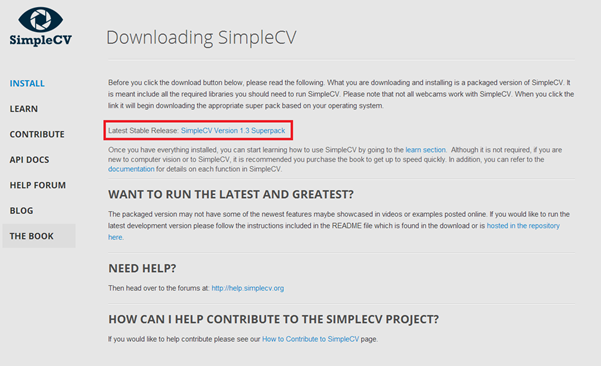
\includegraphics[scale=0.7]{../shared_assets/screenshots/manual/simplecv_download.png}
        \end{figure}

        The files included with the downloaded repository will include an example configuration file called `client.cfg'. As shown
        below in figure~\ref{lst:clientcfg}, this must but set to use values that suite your system needs. To find the `haar\_cascade'
        path you must find where your Python installation resides and check `dist-packages' for the `SimpleCV' folder, then it should
        be under `Features/HaarCascades' as of version 1.3.

        \begin{figure}[H]
            \centering
            \caption{Example client configuration included in code repository.}
            \label{lst:clientcfg}
                \lstinputlisting{../../code/client/client.cfg}
        \end{figure}

        After downloading and installing the relevant `superpack' for your system, you can run the client with Python version 2.7.

    \subsubsection{Server}
        The serv

\section{Tutorial}

    \subsection{Introduction}
        In section I will break down how to use each part of the system in the sections below, each sub-section will include one feature of
        the system explained with detailed text instructions and annotated diagrams to assist you in running the system to its full extent.
    \subsection{Assumptions}
        Assumptions have been made around the proficiency of the user, these include knowing how to start a Python script and having a lot of
        experience previously working with computers.

    \subsection{How do I create a new user?}
        This requires actions on both the server and client, firstly the user must be added to the server database so that the client request 
        succeeds when prompted. This requires running the `db\_browser' and adding a user via the provided user interface, in figure~\ref{fig:dbadduser}
        you can see the `File' menu being opened and a new user dialogue popping up.

        \begin{figure}[H]
            \centering
            \caption{A screenshot of the SimpleCV website where it is possible to download the `superpack'.}
            \label{fig:dbadduser}
                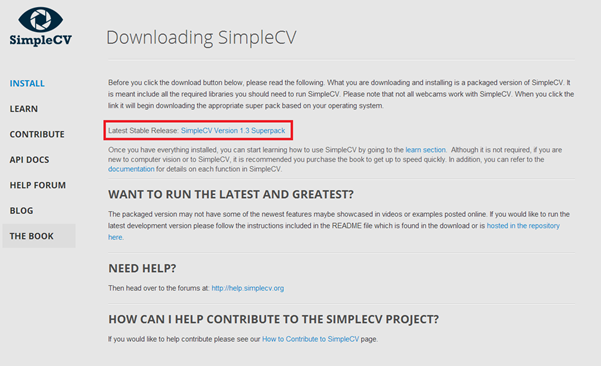
\includegraphics[scale=0.7]{../shared_assets/screenshots/manual/simplecv_download.png}
        \end{figure}

    \subsection{How do I start a new log file?}
    \subsection{How do I check what logs?}
\section{Errors}
    \subsection{SimpleCV/Camera related}
    \subsection{Network related}
    \subsection{Settings}
\section{System Recovery}
    \subsection{Backing up data}
    db\newline
    log files, sqlite database
    client\newline
    user images
    \subsection{Restoring data}

\end{document}
